\documentclass{article}
\usepackage{tikz}
\usetikzlibrary{shapes,arrows}
\usepackage{caption}
\begin{document}
	\begin{titlepage}
    	\title{Master controller definition}
    	\author{Michael King, 200402171}
    	\maketitle
    	\thispagestyle{empty}
	\end{titlepage}
    \begin{abstract}
        The purpose of this document is to define the requirements and provide a
         simple work plan for the Master controller main module. This document 
         will include a simple block diagram, flowcharts for operating modes. And some software design elements.
         \newpage
	\end{abstract}
    \section{Introduction}
        The Master Controller will be the most complex single part of the entire
         project, the purpose of the master controller is to act as a gateway
         between the wired and wireless networks, display errors, provide a
         power supply for wired devices, and provide a simple menu for viewing 
         devices on the network.
     
     \section{System overview}
     The block diagram shown in figure~\ref{fig:simpleblock} is meant to
     encompass the components contained within the enclosure of the Master
     controller main unit. Some simplifications have been made, the A/C
     power supply will be connected to everything. And likely separate from
     the PCB that most of the rest of the components will be located on.
     \begin{figure}[htp]
	     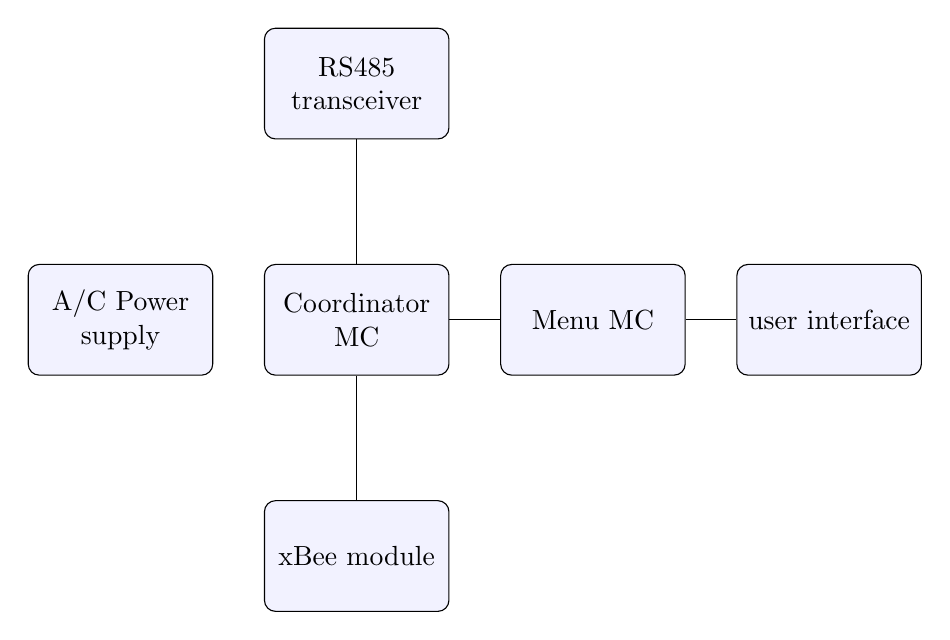
\begin{tikzpicture}[auto, node distance=3cm,>=latex']
    	 	% Define block styles
    	 	\tikzstyle{block} = [rectangle, draw, fill=blue!5, text width=6em, text centered, rounded corners, minimum height=4em]
    	 	\tikzstyle{line} = [draw, -]
    	 	
    	 	% Nodes
    	 	\node [block] (coordinator mc) {Coordinator MC};
    	 	\node [block, right of=coordinator mc] (menu mc) {Menu MC};
    	 	\node [block, below of=coordinator mc] (xBee) {xBee module};
    	 	\node [block, right of=menu mc] (user interface) {user interface};
    	 	\node [block, above of=coordinator mc] (RS485) {RS485 transceiver};
     		\node [block, left of=coordinator mc] (Power Supply) {A/C Power supply};
     	
    	 	% Connecting lines
     		\path [line] (coordinator mc) -- (menu mc);
     		\path [line] (menu mc) -- (user interface);
     		\path [line] (coordinator mc) -- (xBee);
     		\path [line] (coordinator mc) -- (RS485);
     	\end{tikzpicture}
     	\caption{block diagram representing subsystems within the enclosure of the Master Controller}
     	\label{fig:simpleblock}
     \end{figure}
     \newline 
     A decision was made to place separate microcontrollers within the Master Controller to allow
     the coordinator micro to be focuses entirely on coordinating messaging between the wired 
     and wireless networks, while the menu micro only needs to display messages from the coordinator
     and keep track of a device list.
     \newpage
     \section{operations}
     	see figure~\ref{fig:simpleflowRS485RX} for a simplified flowchart of the operation of the Master Controller main unit.
     	\subsection{coordinator}
     		The coordinator's primary task is to perform coordination between the wired and wireless
     		 networks, but it will also filter out system messages to send to the menu controller,
     		 and assign devices on the wired network. And potentially provide collision detection 
     		 for its connected control modules on the wired network.
     		 As such, it needs to be capable of keeping a large amount of device a names in memory for 
     		 quick reference when messages arrive. And have a reasonable buffer for messages.
             We will target having enough memory for at least 1024 wireless devices.
             most likely, this will be a 3.3v device so that it can use the same 
             voltage regulator as the xbee module
     	\subsection{menu}
     		The menu micro spends most of its time listening for system messages from the coordinator 
     		these may be error messages, or other general status (i.e. new device joins network). The 
     		menu micro is responsible for managing the user interface as well.
     	\subsection{user interface}
     		The user interface consists of two parts: some type of display managed by the menu micro, 
     		And some type of user input to navigate through a log of system messages, and a simple 
     		device map.
     	\subsection{power supply}
     		The primary wired A/C power supply may be located within the master controller enclosure, 
     		the purpose of this is to provide power to all wired modules (with the possible exception 
     		of the lap counter display.) This will most likely be a 12v power supply.
     	\subsection{RS 485 Transceiver and xBee module}
     		These serve as the link between the coordinator and the rest of both networks. The xBee 
     		module is constrained to 3.3V. xBee modules provide an expected range
             of nearly 1km, with communication rates in the dozens of kbps.\ while
             RS485 can be expected to have a range of at least 1km, with a data 
             rate in the 100's of kpbs. Both of which should exceed our 
             requirements.
     \begin{figure}[htp]
     	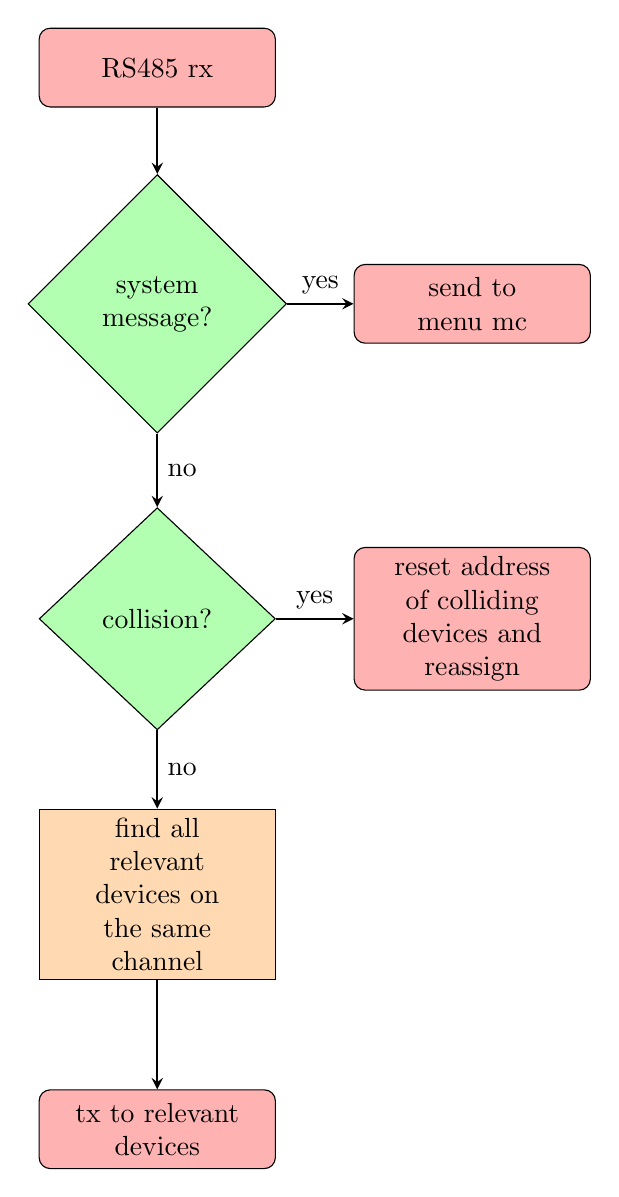
\begin{tikzpicture}[auto, node distance=3cm,>=latex']
     		%define block styles
     		\tikzset{
     			startstop/.style={rectangle, rounded corners, minimum width=3cm, text width=6em, minimum height=1cm, text centered, draw=black, fill=red!30},
     			process/.style={rectangle, minimum width=3cm, minimum height=1cm, text width=6em, text centered, draw=black, fill=orange!30},
     			decision/.style={diamond, minimum width=3cm, minimum height=1cm, text width=6em, text centered, draw=black, fill=green!30},
     			arrow/.style={thick,->,>=stealth},
     			}
     		%define nodes
     		\node[startstop](rx){RS485 rx};
     		\node[decision, below of=rx](errcheck){system message?};
     		\node[startstop, right of=errcheck, xshift=1cm](display){send to menu mc};
     		\node[decision, below of=errcheck, yshift=-1cm](collcheck){collision?};
     		\node[startstop, right of=collcheck, xshift=1cm](reassign){reset address of colliding devices 
            and reassign};
            \node[process, below of=collcheck, yshift=-0.5cm](channel){find all relevant devices 
            on the same channel};
            \node[startstop, below of=channel, yshift=0.5](xBee tx){tx to relevant devices};
            %define arrows
            \draw[arrow] (rx) -- (errcheck);
            \draw[arrow] (errcheck) -- node[anchor=south] {yes} (display);
            \draw[arrow] (errcheck) -- node[anchor=west] {no} (collcheck);
            \draw[arrow] (collcheck) -- node[anchor=south] {yes} (reassign);
            \draw[arrow] (collcheck) -- node[anchor=west] {no} (channel);
            \draw[arrow] (channel) -- (xBee tx);

     	\end{tikzpicture}
     	\caption{RS485 RX flowchart}\label{fig:simpleflowRS485RX}
     \end{figure}
     \subsection{Wired Network Device Types}
     	This system is intended to be very flexible, so this list is not restrictive.
     	\subsubsection{Light controller}
     	Configured to send controls to a single light channel.
     	The pit light is the same unit, just with different coloured buttons and slightly modified code.
     	(include a concept drawing)
     	\subsubsection{Lap counter and controller}
     	The lap counter is expected to be either a gas station price sign, or a crosswalk countdown sign.
     	The lap counter controller is intended for use only on the wired network. (though a wireless version could be easily developed.)
     	The controller includes:
     	\begin{itemize}
     		\item current lap display
     		\item buttons to increment/decrement
     		\item button for last lap "LL"
     		\item button for half way (either wide H, or "HH").
     		\item button to zero out the display
     	\end{itemize}
     	The display also works on the wired network, but could be adapted to be wireless.
     	The display is powered through a separate power supply from the generator. Not through the network cable.
     	\subsubsection{Wired Lights}
     	These are basically the same as the wireless lights, they just have the wireless transceiver replaced with an RS485 one.
     	They take power through a separate power cable, not the network cable.
     \subsection{Error codes and detection}
     as part of the requirement for reliability, The master controller will serve as a point to read error and system status messages sent across the network.
     \subsubsection{Error messaging concept}
     Channel zero could be reserved for errors, and special system messages,
     with the Coordinator unit sending these directly to the attached menu micro.
     Error or system messages should include:
     \begin{enumerate}
     	\item The source device of the report message.
     	\item Error "target", device which has an error.
     	\item Error severity.
     	\item The type of error.
     	\item any additional details.
     \end{enumerate}
     \subsubsection{message types}
     conceptual, add more if beneficial
     \begin{itemize}
     	\item Loss of connection / cannot connect
     	\begin{itemize}
     		\item Critical Error
     		\item Sent by a reporting device
     		\item occurs when a device misses a handshake, or if it never responds to a command
     		\item includes the reporting device, and the device that is not connectable
     	\end{itemize}
     	\item Device internal failure
     	\begin{itemize}
     		\item Critical Error
     		\item Sent by a device with an error
     		\item internal diagnostic reports a failure to function
     		\item includes detail of what failed
     		\item i.e. light 2 green failed to turn on.
     	\end{itemize}
     	\item Battery low
     	\begin{itemize}
     		\item important
     		\item Sent by a device that has detected a low battery status
     		\item could include a time estimate
     	\end{itemize}
     	\item new device connected
     	\begin{itemize}
     		\item advisory
     		\item sent by a device that has newly connected to the network
     		\item includes the device name (if defined), type, and channel.
     		\item i.e "SECTOR 3 LIGHT has joined the network on channel 4 as a wireless light"
     	\end{itemize}
     	
     \end{itemize}
     \section{initial plan}
     Modular, all separate units vs custom all in one. 
     Modular with separate units was selected to help ensure system is easy to expand.
     All, light controllers where initially expected to have 4 buttons (Green, Yellow, Red, Blue).
     This was later changed to only allow the Master controller to set all lights to red. 
     Since only the race director has the authority to stop the race.
     
     (include some diagrams of the modular network concept)
     
     \section{after the first meeting}
     After receiving feedback, The decision was to retain modular units. 
     But to enclose the majority within a single enclosure (include diagram of single enclosure concept). 
     The enclosure has space for one additional sector of light controls that will remain unpopulated initially. 
     The different controls are all still connected through a wired RS485 network. 
     But due to the close proximity, RJ45 jacks may be foregone within the enclosure. 
     With the boards just being directly wired to each other.
     An additional change was made in the form of a move to a single stop button that locks and sets all lights to stop, with individual stop buttons being removed from all devices.
     In order to retain a redundant safety stop, A special portable stop button may be developed for the Race Director to carry at all times.
     
     \subsection{new network concept}
     The network still works mostly the same, just with the majority of devices being  located within a single primary enclosure.
     Future expansions could either modify/enlarge the enclosure,
     or be placed in separate enclosures and connected using a network cable.
     
     \subsection{Primary enclosure design}
     The primary enclosure still contains an A/C power supply. as well as every controller needed for the initial planned network.
     (include diagram)
     \subsection{other changes}
     \begin{itemize}
     	\item The starting line requirements have been updated. 
     	The starting line should now have 3 lights directly beside each other.
     	(include a diagram for this)
     	\item Marshal and light controllers now only need three buttons.
     	\item In order to meet the no single point of failure requirement for our network.
     	We should consider a second wireless controller with a stop light. Maybe a special Race Director handheld controller.
     \end{itemize}
     \section{Central board high level design}
     \subsection{coordinator}
     Ideally, the coordinator will be the same micro that we are already using for everything else.
     But if need be, it can be replaced with something more powerful.
     The coordinator needs to connect to the wired network, the wireless network, and the menu controller.
     All three connections could make use of USARTs.
     \subsection{menu controller}
     This is intended to handle display of errors and user configurable settings through the menu.
     The intent is that this will be capable of displaying a simple network map of connected devices.
     As well as displaying errors and other system messages received from the coordinator.
     This is likely to be the same type of controller as everything else.
     The type of display depends on what we decide on. Likely some kind of simple matrix LCD.
     This controller will also be connected to control panel buttons.
     
     \section{Software high level design}
     \subsection{coordinator}
     The intent with the coordinator software is sequential:
     \begin{enumerate}
     	\item initialize, find and connect to a network. form a network.
     	\item assignment, find all wired devices, starting with counting up any that are already assigned.
     	\item after connecting, enter round-robin communication mode on the wired network. and listen to anything from the wireless or the menu.
     \end{enumerate}
     \subsubsection{initialization}
     The initialization routine includes:
     \begin{itemize}
     	\item any diagnostic we could think of
		\item find or create a network, send out a ping to all devices to start building the list
     	\item wait until it stops receiving devices on the wireless then move to the wired assignment mode
     \end{itemize}
     
     \subsubsection{Wired assignment}
     wired assignment starts by collecting the 8 bit address of devices that are already assigned.
     This occurs one at a time, it will ping all 255 addresses and collect the information on any that respond.
     After finding any already connected devices, it will then send a ping out to any unassigned devices.
     The idea with the auto-learn routine is that each device has a "random" delay between 0 and 1000ms.
     when a device reaches its delay time, it sends a ping back to the master.
     The master collects the information about this device, assigns a semi-permanent ID to it, then sends out another ping.
     Auto-learning could take up to 255 seconds in the worst case. But it only needs to happen the first time the network is assembled.
     So this should still be an acceptable delay.
     While learning, the display should show that it is currently learning and it might take a while.
     It could also show how many wired devices have been detected, and list off any newly assigned devices.
     The device only enters assignment mode on startup, if a new device is added afterwards, then the controller will need to be power cycled.
     (Could also probably be triggered through the menu)
     
     \subsubsection{round robin}
     The master controller pings each device on the wired network in sequence.
     Each device is expected to respond with a short acknowledgment even if there is nothing to report
     , and if nothing is received it will show an error.
     If a device has something to say, it will wait until it is pinged then respond.
     All devices are listening all the time, if they hear something relevant to them then they will process it and come up with a response.
     (in order to deal with multiple devices on the same channel on the same wired network. Maybe other wireless devices could determine what number of responses to expect from a master controller.)
     If a message comes through on the wireless network:
     \begin{enumerate}
     	\item check the channel number, if there are no connected devices on the channel then don't bother broadcasting over the wired network.
     	\item if channel is 0, then send the message to the menu micro.
     	\item otherwise, broadcast the message over the wired network.
     	\item return to round robin mode, relevant devices will come up with a response to that message and respond in turn.
     	The sending device needs to keep track of how many responses it should expect.
     \end{enumerate}
     If a message comes through on the wired network:
     \begin{enumerate}
     	\item check the channel number, if there are no devices on the wireless network in the same channel then don't do anything with the message.
     	\item if the channel is 0, send the message to the menu micro, and broadcast if there are any other master devices.
     \end{enumerate}
     If a message comes from the menu micro:
     \begin{enumerate}
     	\item check the target of the command, if it is meant for a device on the wired network then send it there.
     	\item otherwise broadcast the command over the network.
     \end{enumerate}
     \subsubsection{new wireless device}
     When a new wireless device joins the network, the coordinator needs to:
     \begin{enumerate}
     	\item store the device address, type, and channel
     	\item determine the device type and respond appropriately.
     	\begin{itemize}
     		\item if the device is a controller, then respond with the number of wired targets in the same channel.
     		\item if the device is another master controller, just respond with the address.
     		\item if the device is a target, respond with the number of wired controllers in the same channel.
     	\end{itemize}
     	\item if there are no wired devices on the same channel, just store the device for system wide messages.
     	
     	\item if there are wired devices on the same channel, broadcast the joining message over the wired network so they can add the device to their internal lists.
     	
     	\item after, return to round robin
     \end{enumerate}
     \subsection{menu micro}
     The menu micro manages the display, and the controls.
     \subsubsection{display}
     The display is meant to show errors and general system status messages.
     But could also potentially be used to provide a network map,
      and assign names to devices on the network.
      As well as accessing any other user configurable commands.
     Because of the complex variety of tasks for this display, a touchscreen should be a good choice.
     A touchscreen display would be easy to reconfigure for different applications without making any physical changes.
     And allows for a large amount of information to be displayed and manipulated.
     A nextion display has a built in microcontroller that handles most of the overhead of running the display and touch input.
     But we do not have much access for using this micro to process data,
     so the menu micro will still be responsible for processing data, storing a device list,
     and sending commands to the display micro.
     
     \subsubsection{internal memory}
     The menu micro should also keep track of any devices on the wireless, as well as the wired network.
     It can store any user assigned name, device type and channel as well as the 64 bit ID or 8 bit ID.
     Then this list of stored devices can be displayed on request.
     
     This information could probably be stored in flash, as it wouldn't change often and would only really be accessed on request from the user in the form of the network map.
     
     the device could store the current state of connected devices in RAM, and point to a structure in flash containing the rest of the information.
     
     when it is time to generate the network map, it will go through flash and pull each device.
     It will display the device name, type, current status, and possibly the address as well.
     
     
     \subsubsection{controls}
     The other responsibility of the menu micro is to respond to any of the user control inputs.
     These inputs may come from the Nextion touch screen, or potentially from some other optional general purpose inputs.
     
     \section{alternative coordinator}
     A lighter weight alternative for the coordinator could be made.
     The coordinator doesn't have to create a list of wireless devices if the sending device is responsible for
     knowing where to send things.
     
     \section{hardware design remarks}
     \begin{itemize}
     	\item The nextion display requires a 5 volt supply, so a 5 volt regulator will be selected in addition to the 3.3 volts
     for all the other electronics.
     
     \item When looking into the other boards, an issue was noticed with the original RS485 transceiver in that it's load impedance only
     allowed for a maximum of 32 devices, vs the 256 we had initially intended on.
     This was rectified by replacing it with a direct upgrade that allows for up to 256 devices and has a higher maximum transmission rate.
     
     \item Currently, the primary 12 volt input is making use of a screw terminal. 
     Replacing this with some kind of keyed connector should be considered to avoid an accidental misconnection.
     
     \item in order to prevent potential damage to circuitry from 5v USB power backfeeding.
     A switch will select between the +5v output from the DC-DC converter, or VBUS from the USB port.
     USB2.0 should be able to handle the power requirements of the screen and the rest of the device, and 3.0 is of no concern.
     The switch will also choose between power from the +12v, or power from VBUS for the 3.3 volt converter.
     In this way, the system can be powered either through 12v input, or USB.
     
     \item The nextion display will be mounted separately from the rest of the board, to allow it to be placed optimally.
     This will use a JST XH 4P connector, as it is easily capable of handling the necessary current (approx. 250mA).
     And keyed, so there isn't as much risk of damage occurring due to incorrectly made connections.
     
     \item The nextion display uses a 5 volt TTL level, but it should be capable of working with down to three volt input according to the datasheet.
     It should be possible to use a voltage divider to pull the 5V level down to around 3.3V for the menu microcontroller.
     
     \item A decision was made to include a few GPIO connections to the menu controller on the board.
     This is to allow for potential future controls, even if there isn't any direct plan to use them now.
     They will likely be left without the connectors installed on the board, for potential future use.
     
     \item Since the intent is to also provide power over the twisted pair cable, there should probably be some kind of fusing to protect the cables in the event of a fault.
     The PoE standard specifies a maximum of 300ma per pair, since we intend to use 3 pairs for power we should try to have no more than
     900ma total for the 3 pairs.
     
     \end{itemize}
     \section{selecting a protection device}
     We want this device to be reusable, inexpensive, and small.
     PTC resettable fuses should work well, as they are capable of handling the expected load current.
     And reset automatically once the fault is cleared (eventually).
     \subsection{device sizing}
     with the expected maximum load current of ~900mA, we can select a PTC device with a hold current of 900mA.
     this gives a trip current of 1.8A, and looking at the curve from the datasheet the device should trip within a few seconds at 5A.
     \subsection{device placement} 
     We already have two separate power feeds into the wired network.
     Each with about 11W capability, for a total of 22W in the wired network.
     I will use two PTC devices, and place them in between where power comes in, and where it leaves the master controller board.
     \section{further changes}
     \subsection{coordinator processing}
     Instead of requiring the coordinator to keep track of all devices, we could instead make the sending device responsible for
     knowing the destination addresses and instructing the coordinator to transmit over wireless where applicable.
     This can greatly lighten the processing load on the coordinator as all it really needs to do now is check the channel to see whether it should be sent to the menu or not.
     And check to see if the message should be transmitted over wireless using a supplied address.
     \subsection{on/off, all stop, systemwide commands}
     Instead of having the on/off and other systemwide commands on the main board, they could just make use of another light controller board.
     This would greatly simplify the code of the menu controller, and allow the system-wide controller to perform more checks on the network.
     
\end{document}